\chapter{Theoretical Framework}
\label{ch:theoretical-framework}

Before starting with rehabilitate the main topic, some basic concepts, technical terms and underlying theory has to be explained.
This is important to faster read through the thesis without the need to interrupt the flow of thought.
In the following, a set of established theories and terms is explained which are not directly related to the thesis formulation, but essential to comprehend numerous contexts.

\section{Android UI}
\label{sec:android-ui}


\begin{figure}
    \centering
    \begin{subfigure}[b]{0.5\textwidth}
        \centering
        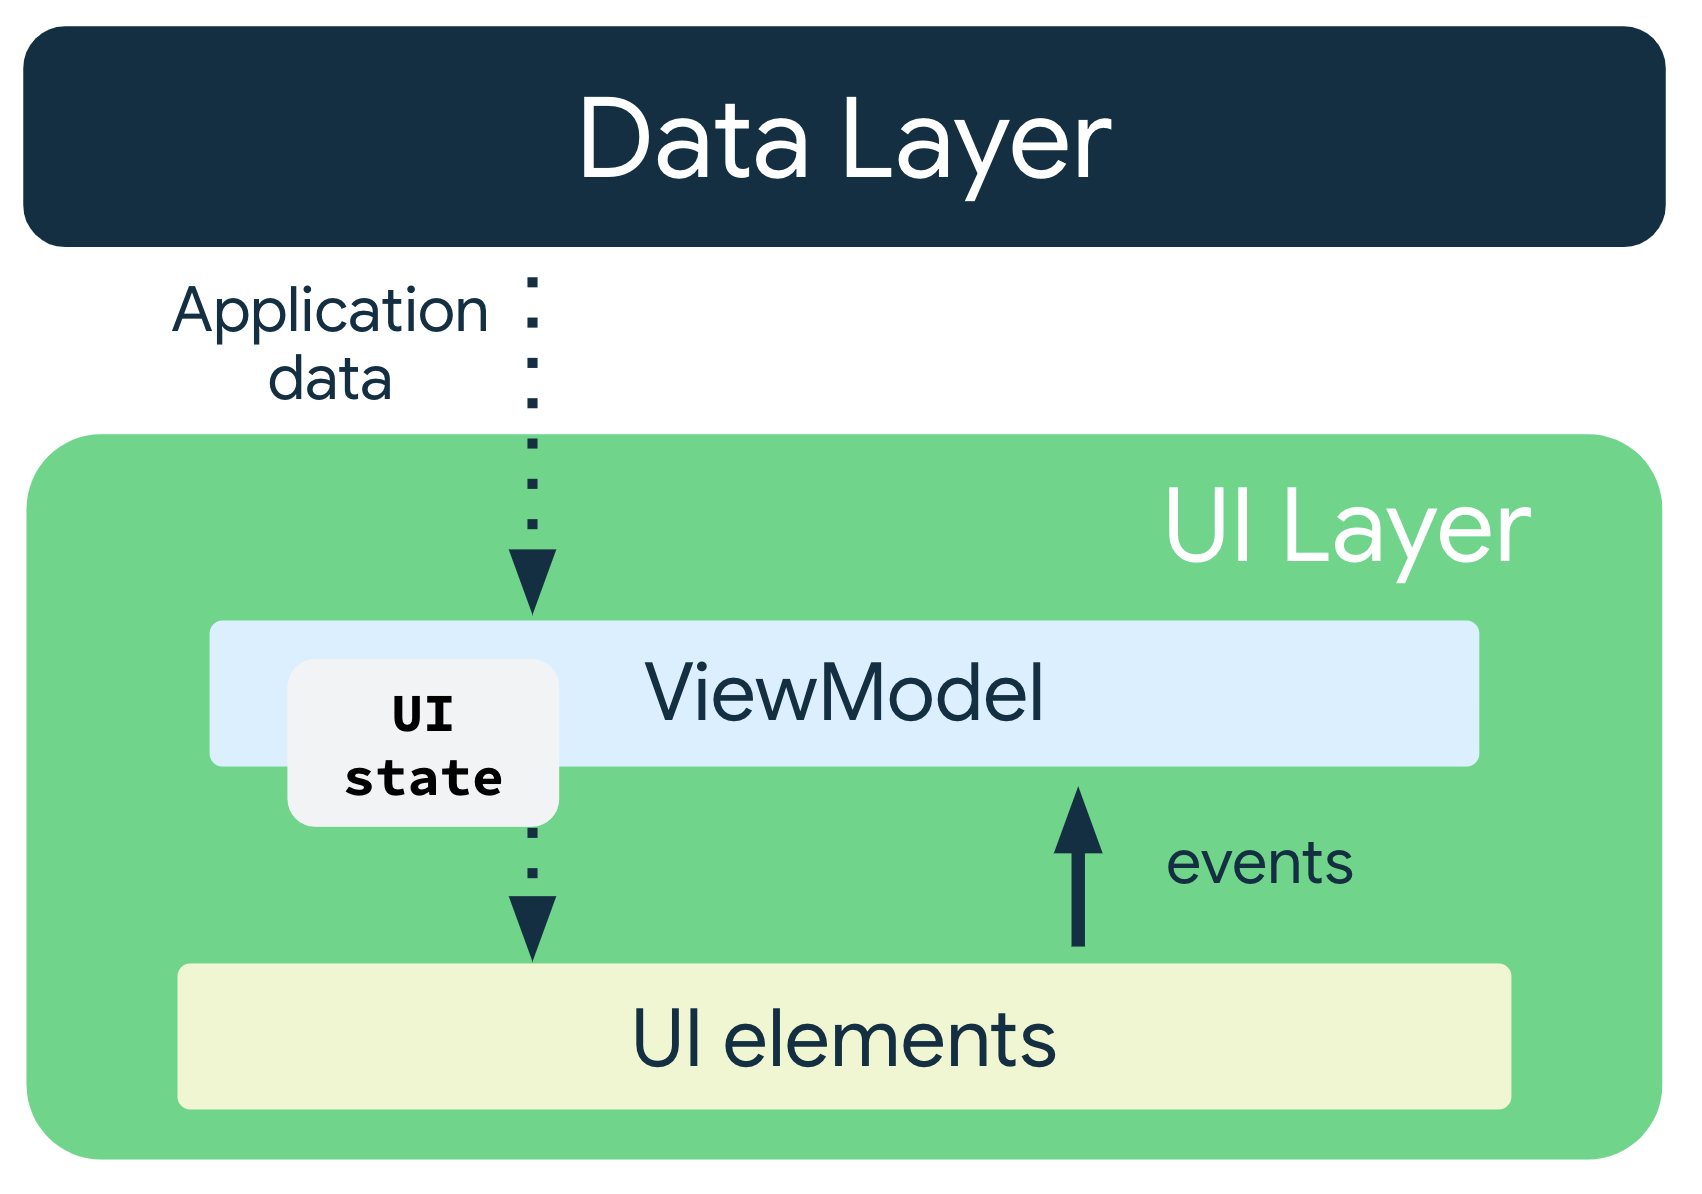
\includegraphics[width=\textwidth]{graphics/android_udf}
        \caption{Diagram of \gls{udf} in app architecture \cite{android_ui_layer}}
        \label{fig:android_udf}
    \end{subfigure}
    \hfill
    \begin{subfigure}[b]{0.4\textwidth}
        \centering
        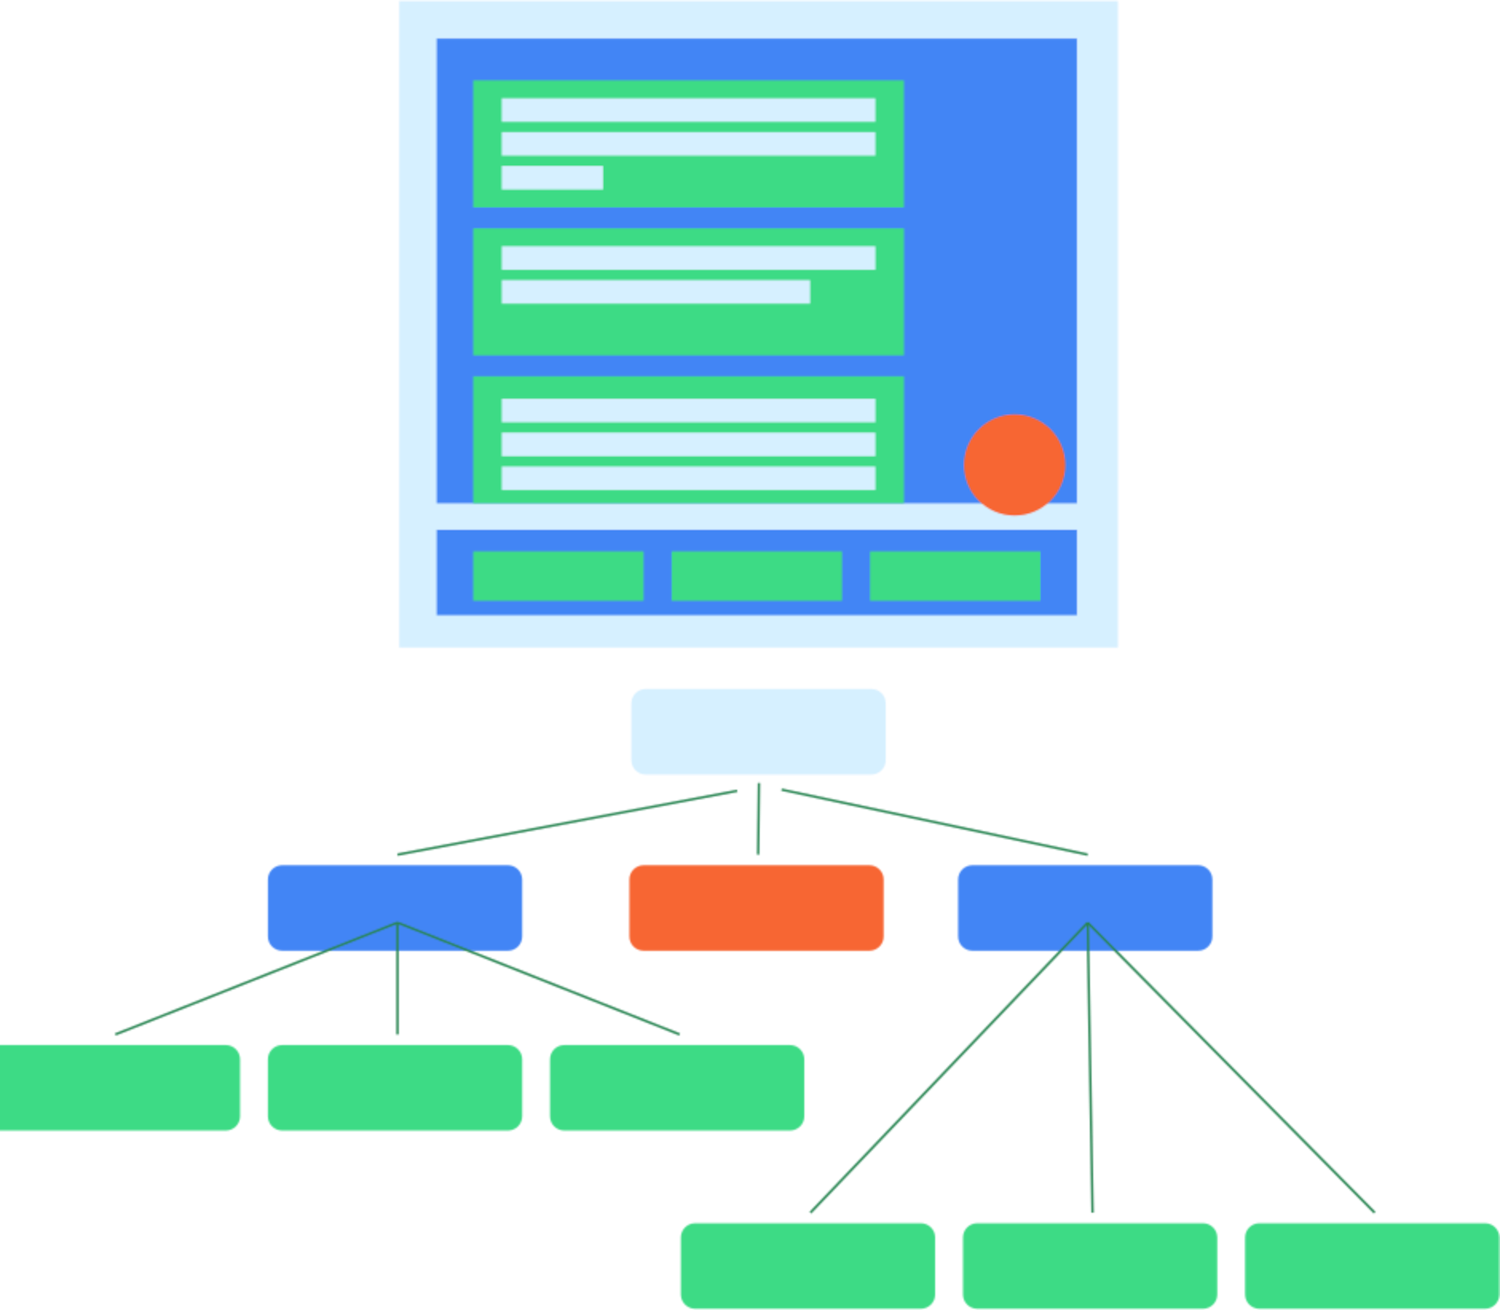
\includegraphics[width=\textwidth]{graphics/android_semantics-ui-tree}
        \caption{Structure of the semantics tree in the UI hierarchy \cite{android_semantics_compose}}
        \label{fig:android_semantics_ui_tree}
    \end{subfigure}
    \caption{Structure of the Android \gls{ui}}
    \label{fig:android_tree}
\end{figure}
https://developer.android.com/topic/architecture/ui-layer \cite{android_ui_layer}
https://developer.android.com/guide/topics/ui/how-android-draws \cite{android_draw_views}
https://developer.android.com/jetpack/compose/mental-model \cite{android_jetpack_compose}

\subsection{Data tree structure}
\label{subsec:data-tree-structure}


Mean 18 actionable elements, with Std=12. \cite{zhou2021large}

\begin{figure}
    \centering
    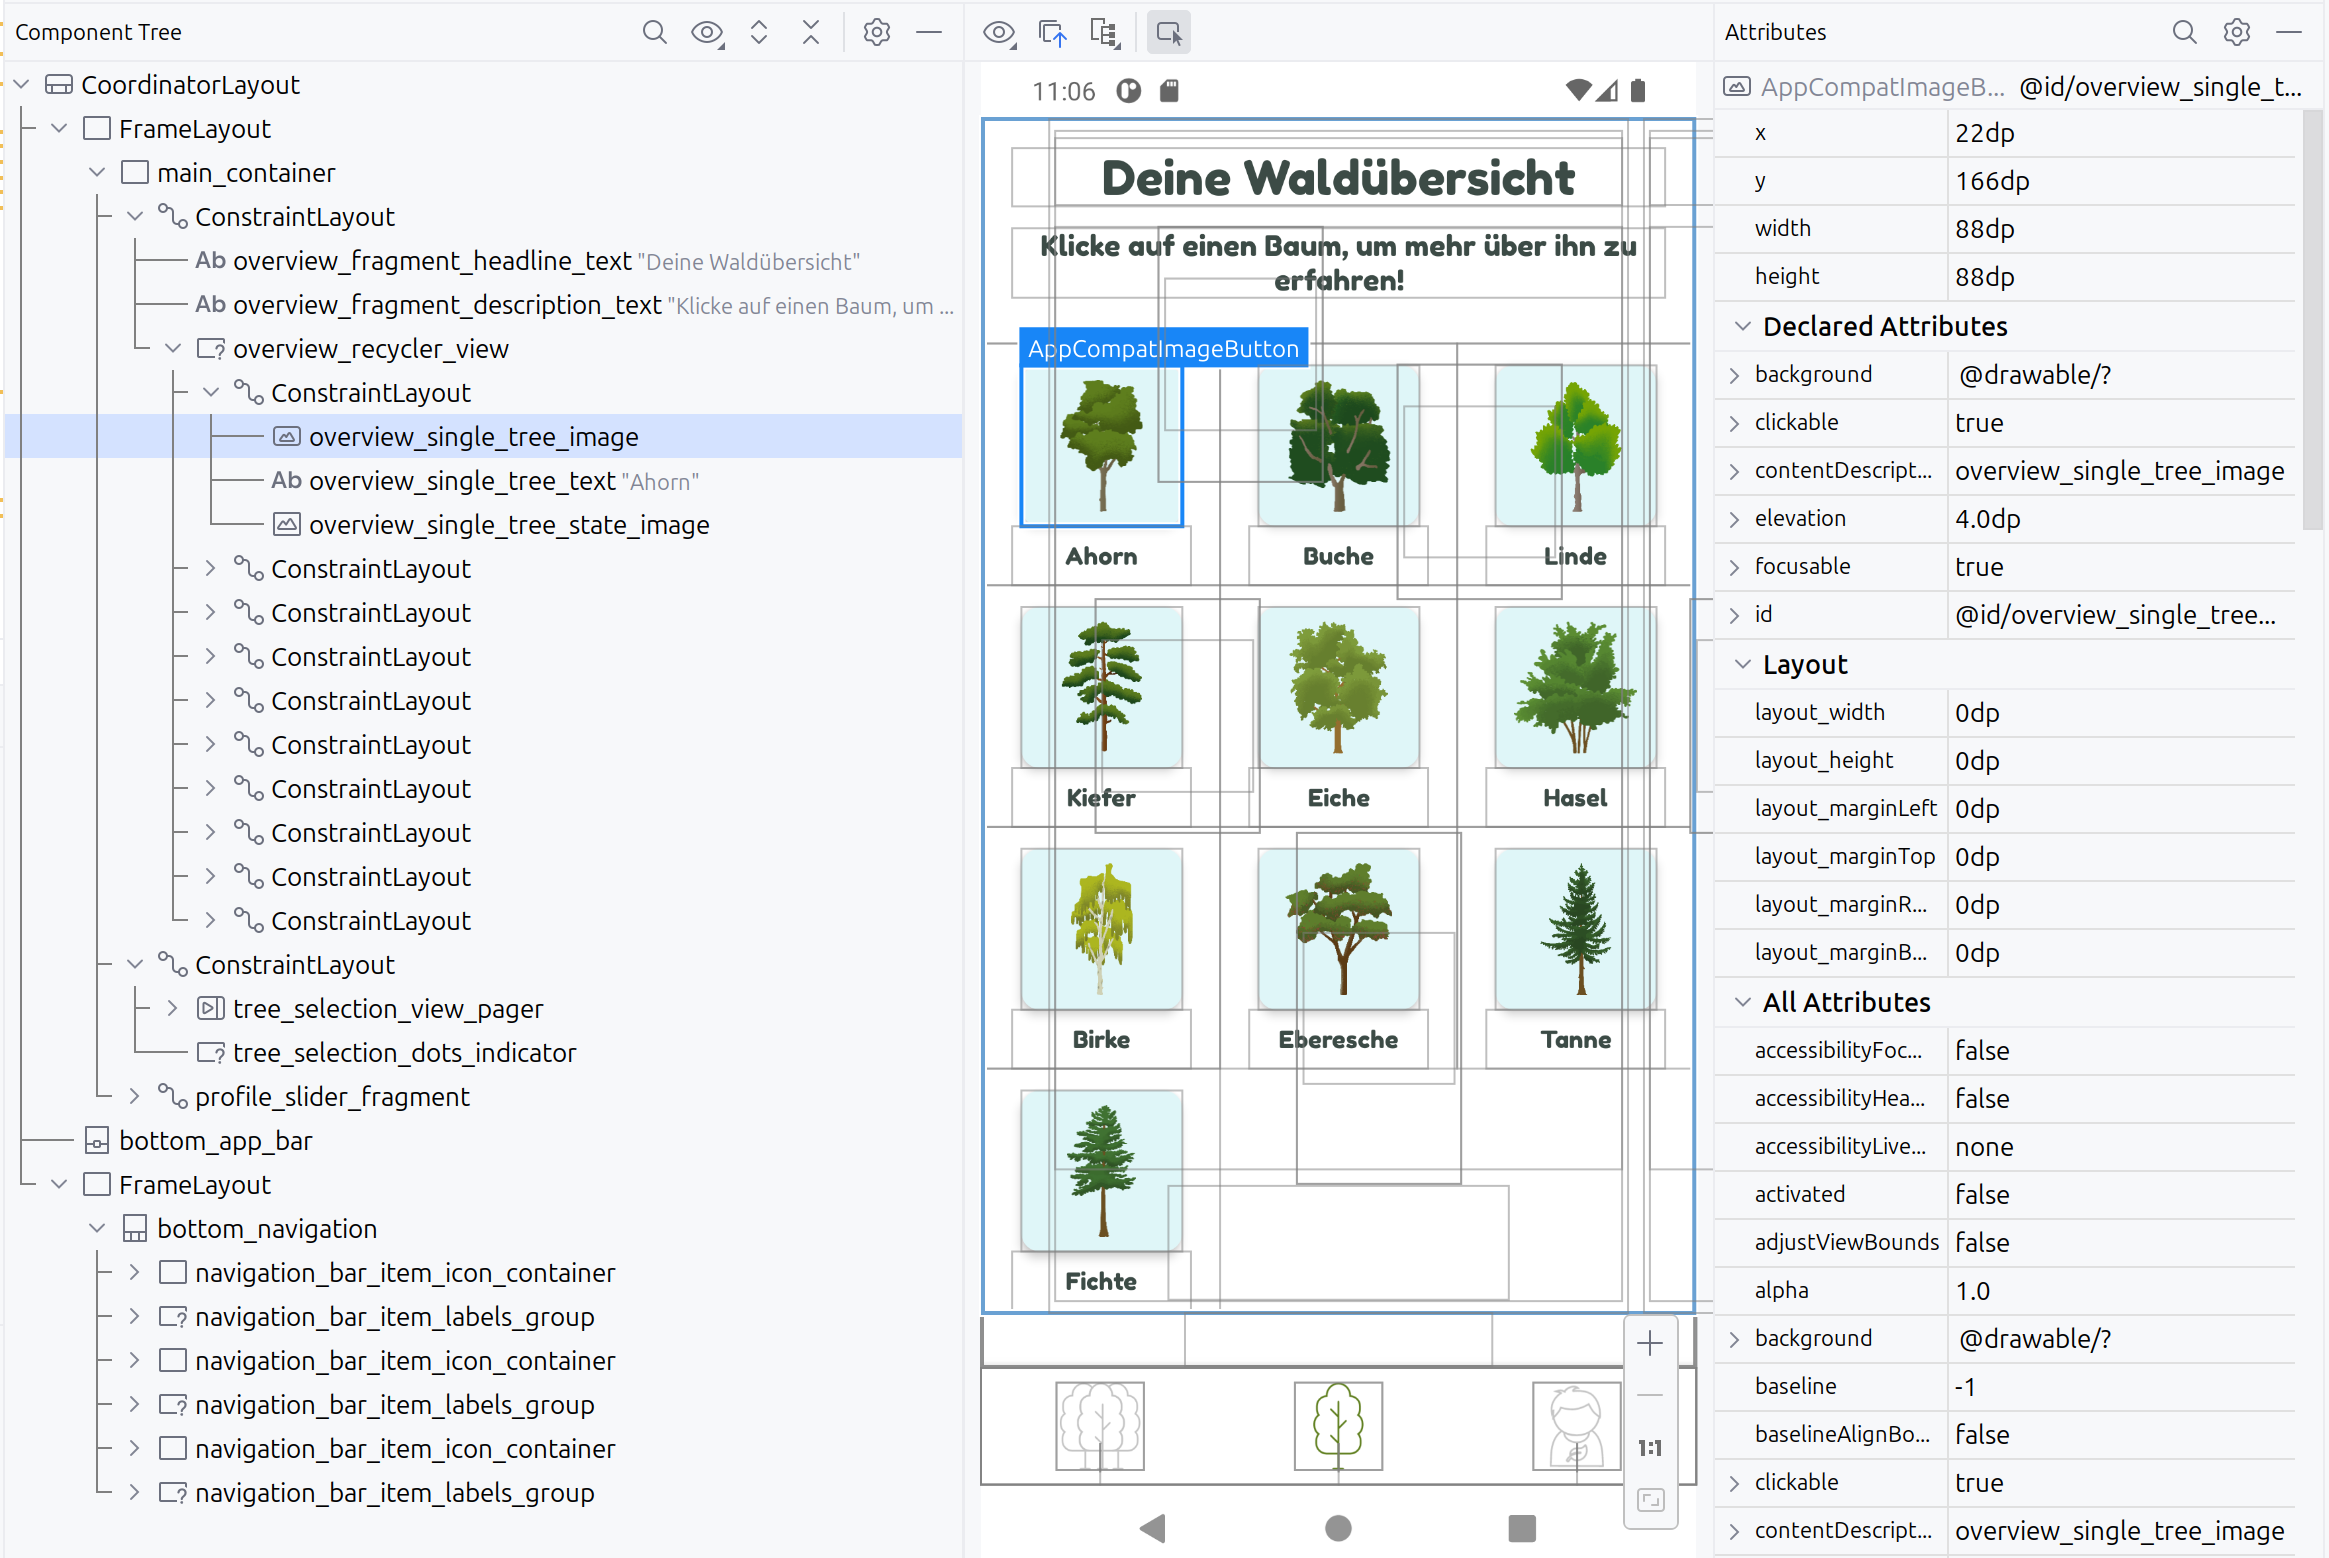
\includegraphics[width=\textwidth]{graphics/android_layout_inspector}
    \caption{\cite{android_layout_inspector}, \cite{mimuc_app_ins_gruene}}
    \label{fig:android_layout_inspector}
\end{figure}

\subsection{Retrieval of UI data via Android Accessibility Service}

Semantics tree:
https://api.flutter.dev/flutter/widgets/Semantics-class.html
https://developer.android.com/jetpack/compose/semantics \cite{android_semantics_compose}
https://android.googlesource.com/platform/frameworks/testing/+/jb-dev/uiautomator/library/src/com/android/uiautomator/core/AccessibilityNodeInfoDumper.java \cite{android_accessibility_node_info_dumper}
%https://github.com/Gustl22/android-accessibility/blob/c158808533d6fc017455184a7317555d3e6946f6/GlobalActionBarService/app/src/main/java/com/example/android/globalactionbarservice/uiautomator/AccessibilityNodeInfoDumper.java

\lstinputlisting[language=XML,label=android_accessibility_node,caption={Android Accessibility Node in XML.},float]{code/android_accessibility_node.xml}

\section{Machine Learning}
\label{sec:machine-learning}

\gls{ml}, a term spread by Arthur Lee Samuel, is a method of data analysis, more precisely a scientific approach to form statistical models without the need to explicitly program it~\cite{mahesh2020machine}.
It uses algorithms to iteratively learn how data is structured.
In contrast to statistical inference or manually crafted statistical models respectively, \gls{ml} can solve tasks by automation of model building.
Its advantages lie in finding hidden relations and patterns from the context, without having any or only a small pre knowledge of the data, thus it is a strong tool for generalization or abstraction of large datasets, also known as \gls{gl-bigdata}.
\gls{ml} can be applied to the following fields among others: email and spam filtering, fraud detection, cybersecurity, web search engines, recommender systems (like known from Netflix or Amazon), advertising, translators and text generation, pattern and image recognition.
The data driven approach also comes with some drawbacks: the outcome heavily depends on the provided data.
It can include biases and therefore may acquire forms of discrimination or unfair treatment.
Nonetheless \gls{ml} has a lot of potential to uncover hidden connections in large datasets.

\subsection{Preprocessing}

Preprocessing describes the step after one acquired their data, but before training the \gls{ml} model.
This step is not to be underestimated.
A \gls{ml} model can perform significantly better when certain preprocessing steps are applied \cite{alam2019impact}.

To be able to preprocess the data, we have to know with what kind of data we handle with.
Data can occur in different forms, but we can break them down in three main types:
\begin{itemize}
    \item \tb{Categorical values}: a value is always assigned to a class with fixed pool of predetermined classes.
          E.g.\ letters, words, brands, animals, chemical elements
    \item \tb{Continuous values}: the value can be fractional and may lies in between a lower and an upper bound.
          E.g.\ temperature, velocity, geographic position
    \item \tb{Integer values}: the value is a whole number and may also lie in between a lower and an upper bound.
          E.g.\ revolutions per minute, product number, annual sales
\end{itemize}

For discrete and continuous values, we have a wide variety of options to prepare them to be able to be processed by a \gls{ml} model \cite{duong2021}.

\todo{Tensors, Datasets}
%https://stackoverflow.com/a/48599383/5164462

\subsubsection{Feature selection}
Such as Filtering privacy invasive details

Parameterizing the vectorization process
a) Vector length
b) Weighting of features
c) Manipulating individual parameters of model

\subsubsection{Missing data}
Some data entries may are missing.
Therefore, you have two approaches to get around these missing values.
One can drop these values by removing the column or row.
This is only recommended if you are not relying on this data entry, or this the whole feature is not expected to be important enough to bring any value to the model's performance.
Further you can fill the data with a default value like zero or calculate a reasonable value from the surrounding data entries by taking their \quotes{mean, median, or interpolation}~\cite{duong2021}.
The second approach can only be applied to numerical data.

\subsubsection{Normalization and Standardization}

This is only applicable for numerical data.
Many \gls{ml} models work better or exclusively with normalized data.
This means that the values have to be in a certain range, most commonly are from \tb{0} to \tb{1} or from \tb{-1} to \tb{1}.
This can be achieved by dividing all values with the difference of the minimum and maximum value and shift the output accordingly \cite{duong2021}.

% X new = (X — X min)/ (X max — X min)

Sometimes this is not enough, e.g.\ if having a few extreme values, and an approach is desired which better reflects the average data.
Here the standardization, also called z-score normalization, comes into play.
This method scales the values so that the mean value is placed at \tb{0} and the standard deviation is placed at \tb{1}.
%https://medium.com/analytics-vidhya/what-are-data-standardization-and-data-normalization-f880dd9e79b6
\subsubsection{Padding}


\subsubsection{Categorical Variables}

\todo{categorical}
According to \cite{alam2019impact} these steps can be removal of emoticons, elimination of stopwords and stemming for text based models.

Category Embedding before LSTM
% https://stackoverflow.com/questions/47217151/keras-lstm-with-embedding-layer-before-lstm-layer
% https://stackoverflow.com/questions/52627739/how-to-merge-numerical-and-embedding-sequential-models-to-treat-categories-in-rn/52629902#comment136040845_52629902


- Embedding layer
Dimension near the actual average length of features (?)

\subsection{Supervised vs Unsupervised vs Semisupervised}

\subsubsection{Supervised Learning}
Supervised: Classification and regression
Uses \tb{labeled} examples: Input and output is known

Learns by comparison of the output it is provided with the output the model \ti{predicts}.

Steps:
- Data acquisition
- Data cleaning / Preprocessing (Panadas)
- Split into Training Data, Validation data, and Test data (cannot adapt the model after using the test data)
- Train the model with the train data
- Evaluate the model with the test data, then can adapt the model by the developer
- Last deploy the model to production

\subsubsection{Unsupervised Learning}
Clustering
Reinforcement learning

self-supervised

\subsection{Under and Overfitting}
\label{subsec:under-and-overfitting}


\section{Artificial Neural Nets}
\label{sec:artificial-neural-nets}

- Uses biological neuron systems as paradigm to generate mathematical models
- can solve tasks by abstraction or generalization of data relations


Activation Functions
Cost function
Gradient
- Regression: Continous Values
- Classification: Multiple class
- One Class

\subsection{Classes of Neural Nets}

\subsubsection{Deep Neural Nets}

Neural Net with more than one layer
- Dense Layer

\subsubsection{Convolutional Neural Nets}
\subsubsection{Recurrent Neural Networks and LSTMs / GRU}
LSTM 4 dimensional
% https://stackoverflow.com/questions/54743549/is-it-possible-to-making-lstm-model-with-4-dimension-shape-of-data

Limitations to only 3 dimensions, needs flattening

Sample dimension (X -> y)
Time (Step) Dimension
Feature Dimension
Data, Quantity dimension, such as Image dimensions, or multiple nodes

TimeDistributedLayer
% https://stackoverflow.com/a/61588937/5164462
% https://stackoverflow.com/questions/53107126/what-are-the-uses-of-timedistributed-wrapper-for-lstm-or-any-other-layers

\subsubsection{Autoencoders}
\label{subsubsec:autoencoder}

Encoder, Decoder

\subsection{Tensorflow and Keras}
Layers
FlattenLayer

Positive Integer to Dense Vectors of fixed size

\section{Evaluation and Metrics}
\subsection{Mean Squared Error}
\subsection{F1 Score}
